\documentclass[15pt]{article}
\usepackage[utf8]{inputenc}
\usepackage[spanish]{babel}
\usepackage{amsmath}
\usepackage{amsthm}
\usepackage{amssymb}
\usepackage{fancyhdr}
\usepackage[margin=0.9in]{geometry}
\usepackage{listings}
\usepackage{listingsutf8}
\usepackage{algorithm}
\usepackage{url}
\usepackage{graphicx}
\usepackage{minted}

\usepackage[export]{adjustbox}

\graphicspath{./}
\pagestyle{fancy}
\lhead{Práctica 4: Servidor HTTP}
\rfoot{\thepage}
\lfoot{ESCOM-IPN}
\renewcommand{\footrulewidth}{0.5pt}
\bibliographystyle{IEEEtran}

%opening
\title{Práctica 4: Servidor HTTP}
\author{3CM7}
\date{3 de diciembre de 2018}

\begin{document}
	
	\begin{titlepage}
		\begin{center}
			
			% Upper part of the page. The '~' is needed because \\
			% only works if a paragraph has started.
			
			\noindent
			\begin{minipage}{0.5\textwidth}
				\begin{flushleft} \large
					
\includegraphics[width=0.3\textwidth]{ipn.png}
				\end{flushleft}
			\end{minipage}%
			\begin{minipage}{0.55\textwidth}
				\begin{flushright} \large
					
\includegraphics[width=0.7\textwidth]{escom.png}
				\end{flushright}
			\end{minipage}
			
			\textsc{\LARGE Instituto Politécnico Nacional}\\[0.5cm]
			
			\textsc{\Large Escuela Superior de Cómputo}\\[1cm]
			
			% Title
			
			{ \huge Práctica 4: Servidor HTTP \\[1cm] }
			
			{ \Large Unidad de aprendizaje: Aplicaciones para comunicaciones en red} \\[1cm]
			
			{ \Large Grupo: 3CM7 } \\[1cm]
			
			\noindent
			\begin{minipage}{0.5\textwidth}
				\begin{flushleft} \large
					\emph{Alumnos:}\\
					\begin{itemize}\setlength\itemsep{0em}
						\item Ontiveros Salazar Alan Enrique
						\item Sánchez Valencia Sergio Gabriel
					\end{itemize}
				\end{flushleft}
			\end{minipage}%
			\begin{minipage}{0.5\textwidth}
				\begin{flushright} \large
					\emph{Profesor:} \\
					Moreno Cervantes Axel Ernesto
				\end{flushright}
			\end{minipage}
			
			\vfill
			
			% Bottom of the page
			{\large 3 de diciembre de 2018}
		\end{center}
	\end{titlepage}

	\maketitle

	\section{Marco teórico}
		\subsection{Protocolo HTTP}
			El \emph{Protocolo de Transferencia de Hipertexto (HTTP)} es un protocolo en la capa de aplicación para transmitir documentos de hipermedia, tales como páginas HTML. Se diseñó para la comunicación entre navegadores Web y servidores, pero se puede usar para otros objetivos. HTTP sigue el clásico modelo cliente-servidor, en donde el cliente abre la conexión para realizar una solicitud, y espera hasta que recibe una respuesta del servidor. HTTP es un protocolo sin estado, lo que significa que el servidor no guarda ninguna información (estado) entre las solicitudes. A pesar de que está basado en la capa de transporte TCP/IP, se puede usar en cualquier otra capa de transporte, como UDP.
		
		\subsection{Estructura del mensaje HTTP}
			Un \emph{mensaje HTTP} es la forma de intercambiar datos entre un servidor y un cliente. Hay dos tipos: solicitudes (\emph{requests}) enviadas por el cliente para realizar una acción en el servidor; y respuestas (\emph{responses}) enviadas desde el servidor al cliente.
			
			Los mensajes están compuestos de información textual codificada en ASCII, que ocupa varias líneas. En la versión HTTP/1.1 y anteriores, estos mensajes se envían totalmente a través de la conexión. En HTTP/2, estos se dividen en tramas HTTP, optimizando más. En esta práctica solo implementaremos HTTP/1.1.
			
			Los webmasters y desarrolladores raramente manejan desde cero estos mensajes HTTP, ya que algún software, navegador, proxy o servidor realiza esta acción.
			
			\begin{figure}[H]
				\centering
				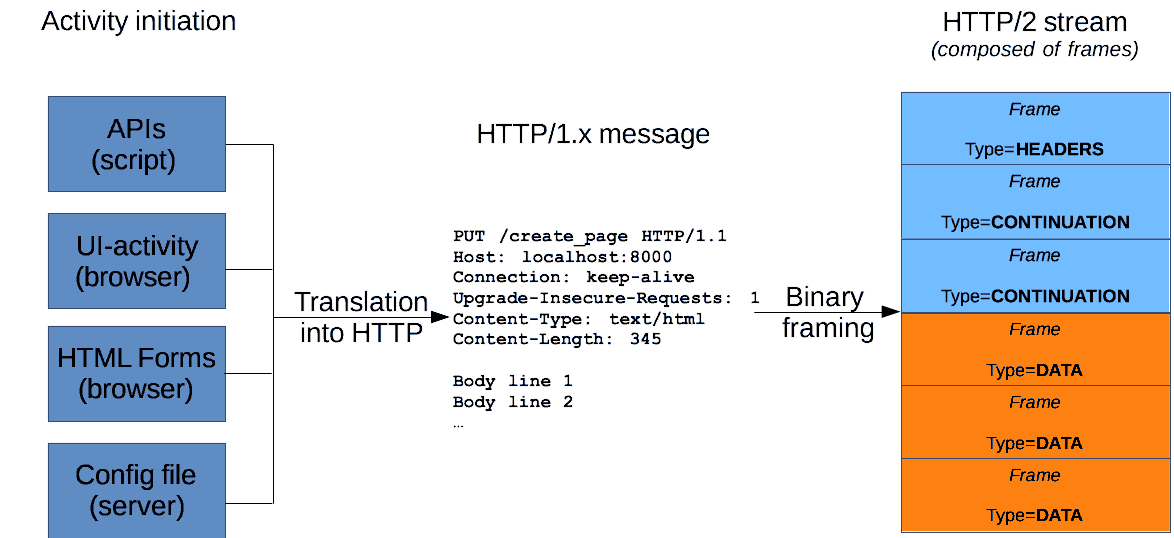
\includegraphics[scale=0.4]{overview.png}
				\caption{Ejemplo general de la estructura de un mensaje HTTP}
			\end{figure}
			
			Las solicitudes y respuestas HTTP siguen un formato de estructura similar entre sí, compuesto de:
			\begin{enumerate}
				\item Una sola línea de comienzo que describe la solicitud a realizar, o el estado de si una solicitud fue exitosa o falló.
				\item Un conjunto opcional de cabeceras (\emph{headers}) HTTP especificando más a detalle la solicitud, o describiendo el cuerpo del mensaje en la respuesta.
				\item Una línea en blanco que indica que toda la información previa (\emph{meta-information}) se ha enviado. Estas líneas usan los caracteres \texttt{$\backslash$ r $\backslash$ n} como separador.
				\item Un cuerpo (\emph{body}) opcional, que contiene los datos asociados a la solicitud (como el contenido de un formulario HTML), o el documento asociado a la respuesta. La presencia del cuerpo y su tamaño se indican con la línea de inicio y los encabezados.
			\end{enumerate}
			
			\begin{figure}[H]
				\centering
				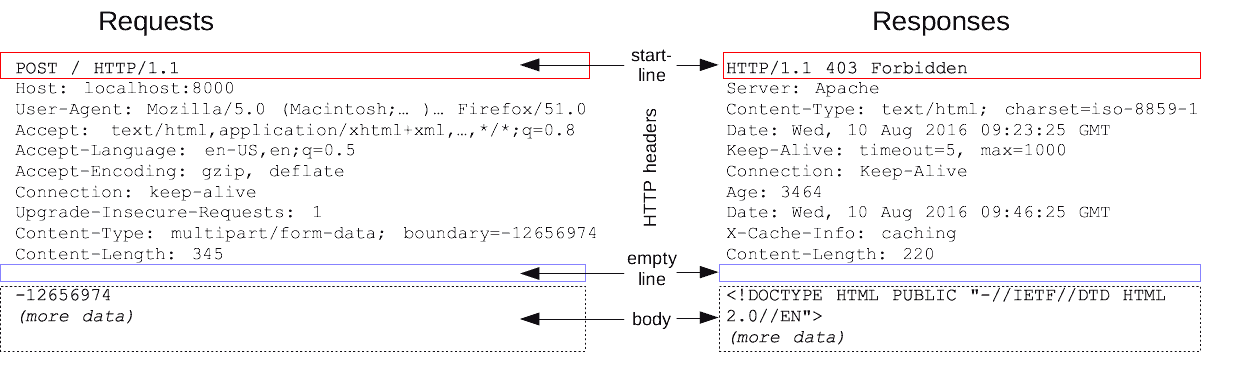
\includegraphics[scale=0.4]{message.png}
				\caption{Ejemplo de una solicitud y una respuesta}
			\end{figure}
			
		\subsection{Solicitudes}
			Son mensajes enviados por el cliente para iniciar una acción en el servidor.
			
			\subsubsection{Primer línea}
			La primer línea contiene tres elementos:
			\begin{enumerate}
				\item El \emph{método HTTP}, que es un verbo que puede ser \texttt{GET}, \texttt{POST}, \texttt{PUT} o \texttt{DELETE}; o un sustantivo, como \texttt{HEAD} o \texttt{OPTIONS}, que describe la acción a realizarse. Por ejemplo, \texttt{GET} indica que se debe devolver un recurso, y \texttt{POST} que se debe enviar datos al servidor.
				\item La \emph{URL} de destino o la ruta absoluta del protocolo, puerto y dominio. El formato puede variar:
				\begin{itemize}
					\item Una ruta absoluta, opcionalmente seguida de un \texttt{?} y un \emph{query string}. Es la forma más común, y se usa con \texttt{GET}, \texttt{POST}, \texttt{HEAD} y \texttt{PUT}. Ejemplos:
					\begin{itemize}
						\item \texttt{POST / HTTP/1.1}
						\item \texttt{GET /background.png HTTP/1.0}
						\item \texttt{HEAD /test.html?query=alibaba HTTP/1.1}
						\item \texttt{OPTIONS /anypage.html HTTP/1.0}
					\end{itemize}
					\item Una URL completa, se usa comúnmente con un proxy. Ejemplo: \texttt{GET http://developer.mozilla.org/en-US/docs/Web/HTTP/Messages HTTP/1.1}
				\end{itemize}
				\item La versión de HTTP, usualmente \texttt{HTTP/1.1}.
			\end{enumerate}
			
			\subsubsection{Encabezados}
			Son elementos del tipo \texttt{clave: valor}. Permiten mandar información adicional con la solicitud. Hay varios tipos:
			\begin{enumerate}
				\item Generales: aplican al mensaje como un todo.
				\item Encabezados de solicitud: modifican la solicitud. Algunos ejemplos son \texttt{User-Agent}, \texttt{Accept-Language}, \texttt{Referer}, etc.
				\item Encabezados de entidad: aplican al cuerpo del mensaje, como \texttt{Content-Length}.
			\end{enumerate}
			
			\begin{figure}[H]
				\centering
				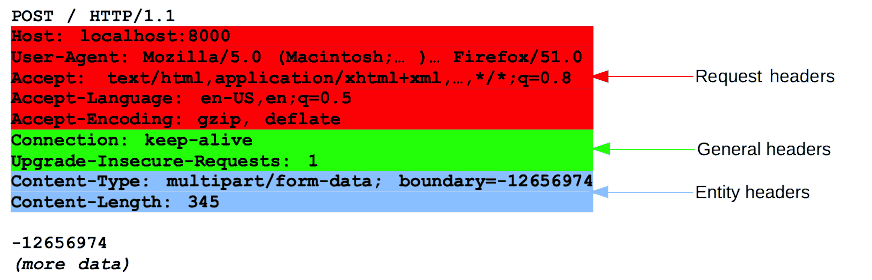
\includegraphics[scale=0.4]{headers.png}
				\caption{Ejemplo de los encabezados más comunes}
			\end{figure}
			
			\subsubsection{Cuerpo}
			Es la parte final de la solicitud. No todas las solicitudes lo tienen, tales como las que solo solicitan recursos, como \texttt{GET}, \texttt{HEAD}, \texttt{DELETE} o \texttt{OPTIONS}.Algunas solicitudes envían datos al servidor para actualizarlo, como es el caso de \texttt{POST}. Los cuerpos de las solicitudes se clasifican en:
			\begin{itemize}
				\item De recurso único: consisten de un solo archivo, definido con los encabezados \texttt{Content-Type} y \texttt{Content-Length}.
				\item De múltiples recursos: consisten de un cuerpo multiparte, cada uno conteniendo una parte diferente de la información. Usualmente se asocia con los formularios HTML.
			\end{itemize}
			
		\subsection{Respuestas}
			\subsubsection{Línea de estado}
			La primera línea de una respuesta HTTP contiene la siguiente información:
			\begin{itemize}
				\item La versión del protocolo HTTP, usualmente \texttt{HTTP/1.1}.
				\item El código numérico de estado, indicando si la solicitud fue exitosa o no. Los más comunes son \texttt{200 (OK)}, \texttt{404 (Not Found)}, \texttt{302 (Found)} o \texttt{500 (Internal Server Error)}.
			\end{itemize}
			
			\subsubsection{Encabezados}
			Tienen el mismo formato que los encabezados de solicitud. Se dividen en:
			\begin{enumerate}
				\item Generales: aplican a todo el mensaje.
				\item De respuesta: proporcionan información adicional sobre el servidor que no caben en la primera línea, como \texttt{Vary} o \texttt{Accept-Ranges}.
				\item De entidad: aplican al cuerpo del mensaje, tales como \texttt{Content-Length}.
			\end{enumerate}
			
			\begin{figure}[H]
				\centering
				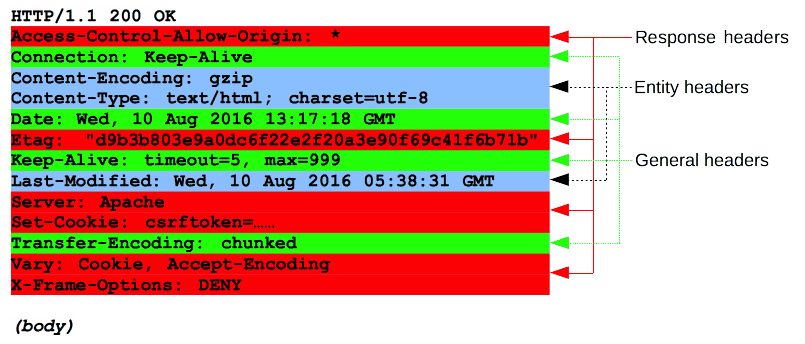
\includegraphics[scale=0.4]{response.png}
				\caption{Ejemplo de una respuesta HTTP}
			\end{figure}
			
			\subsubsection{Cuerpo}
			Es la última parte de la respuesta. No todas tienen uno, por ejemplo, las que tienen como código de error \texttt{201} o \texttt{204}. Se clasifican en:
			\begin{itemize}
				\item De un solo recurso: consisten de un solo archivo de longitud conocida, definido en los encabezados \texttt{Content-Type} y \texttt{Content-Length}.
				\item De un solo recurso con longitud desconocida: consisten de un solo archivo pero no se sabe su tamaño, se usa el encabezado \texttt{Transfer-Encoding: chunk}.
				\item De múltiples recursos: consisten en varios archivos, cada uno contiene distinta información. Casi no es común este tipo.
			\end{itemize}
	
	\section{Desarrollo}
		En esta práctica implementaremos un servidor HTTP 1.1 sencillo corriendo sobre el puerto \texttt{8888}, que soporte los métodos \texttt{GET}, \texttt{POST}, \texttt{HEAD}, \texttt{PUT} y \texttt{DELETE}. Soportará los encabezados más sencillos, tales como \texttt{Content-Length}, \texttt{Content-Type}, \texttt{Date} y \texttt{WWW-Authenticate}.
		
		Tendrá como códigos de error los más comunes: \texttt{404 (Not Found)}, \texttt{403 (Forbidden)}, \texttt{200 (OK)}, \texttt{401 (Unauthorized)} y \texttt{201 (Created)}.
		
		Soportará el examen de directorios con previa autenticación, así como el borrado y subida de archivos (no se permite borrado de directorios).
		
		Además, para solicitudes \texttt{GET} y \texttt{POST}, las páginas \texttt{.html} podrán contener al estilo PHP las expresiones \texttt{<?\_\_GET["key"]?>} y \texttt{<?\_\_POST["key"]?>}, las cuales el servidor se encargará de sustituir con los valores en la solicitud del mensaje.
		
		El documento predeterminado para carpeta será \texttt{index.html}.
		
		Por último, tendremos una alberca de hilos con capacidad de 3 cada vez que se conecte un cliente, esto con el fin de no saturar el servidor.
	
	\clearpage
	\section{Pruebas}
		Corremos el servidor:
		\begin{figure}[H]
			\centering
			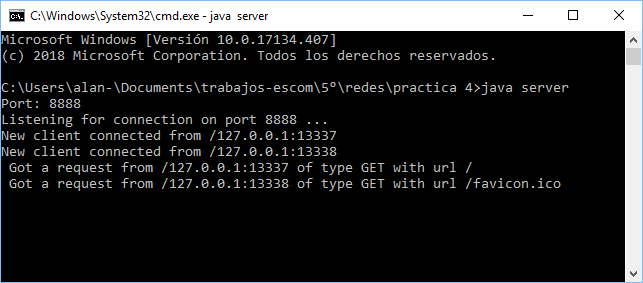
\includegraphics[scale=1]{console.png}
		\end{figure}
		
		\clearpage
		Abrimos un navegador y solicitamos la página principal:
		\begin{figure}[H]
			\centering
			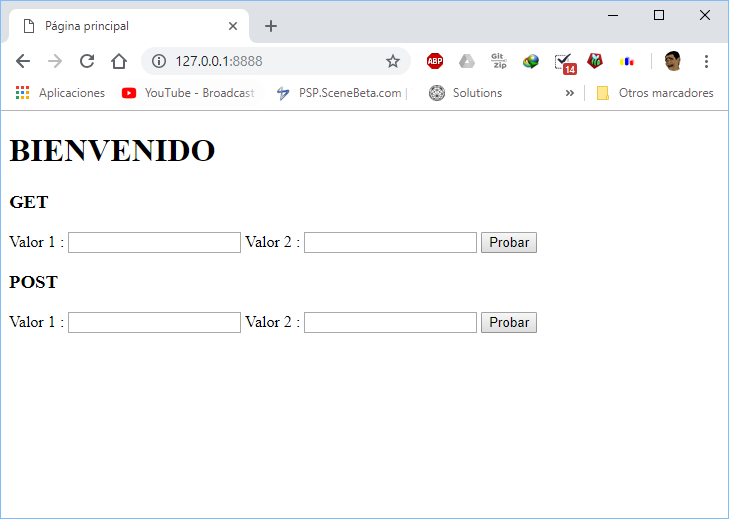
\includegraphics[scale=0.9]{prueba1.png}
		\end{figure}
		
		\clearpage
		Nos logueamos:
		\begin{figure}[H]
			\centering
			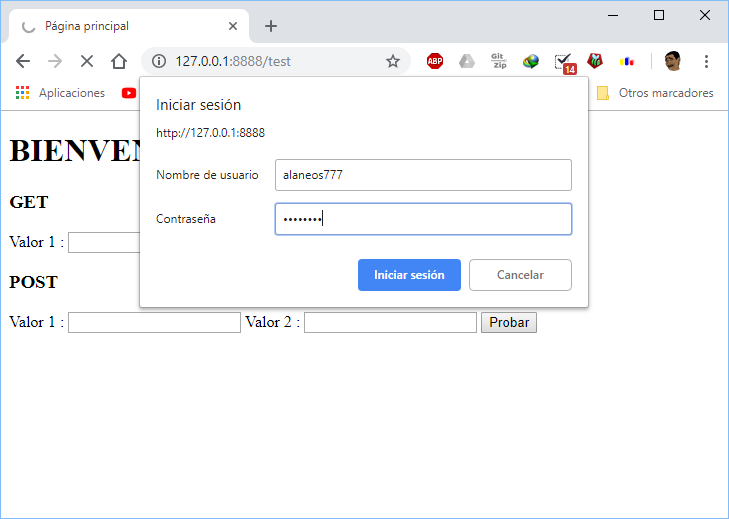
\includegraphics[scale=0.9]{prueba2.png}
		\end{figure}
		
		\clearpage
		Probamos el examen de directorios:
		\begin{figure}[H]
			\centering
			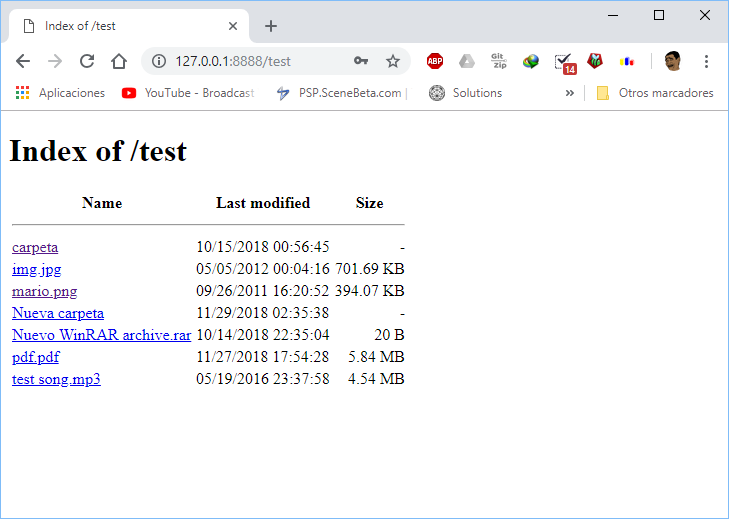
\includegraphics[scale=0.9]{prueba3.png}
		\end{figure}
		
		\clearpage
		Vemos una imagen:
		\begin{figure}[H]
			\centering
			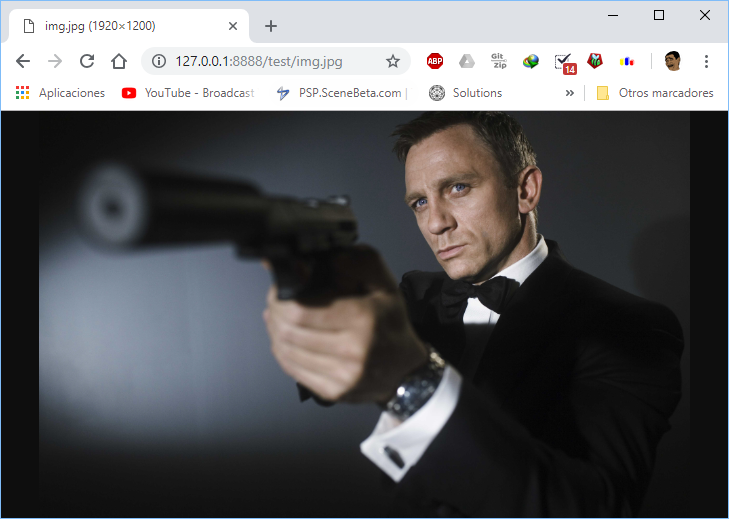
\includegraphics[scale=0.9]{prueba4.png}
		\end{figure}
		
		\clearpage
		Descargamos un archivo más pesado:
		\begin{figure}[H]
			\centering
			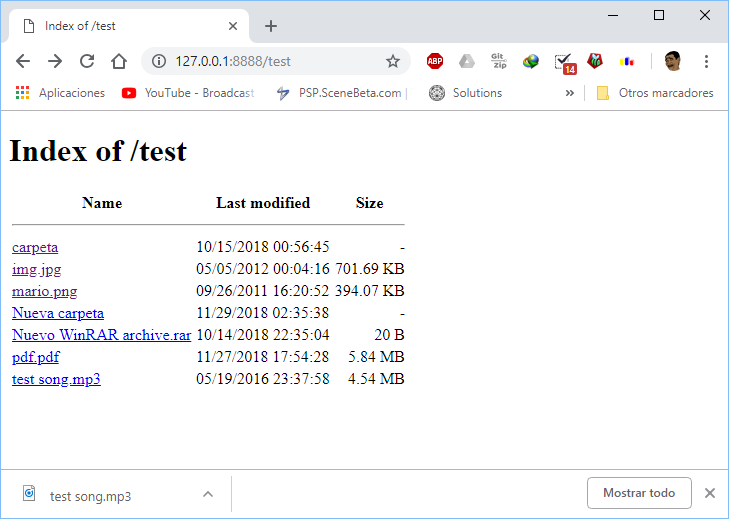
\includegraphics[scale=0.9]{prueba5.png}
		\end{figure}
		
		\clearpage
		Prueba del método \texttt{GET}:
		\begin{figure}[H]
			\centering
			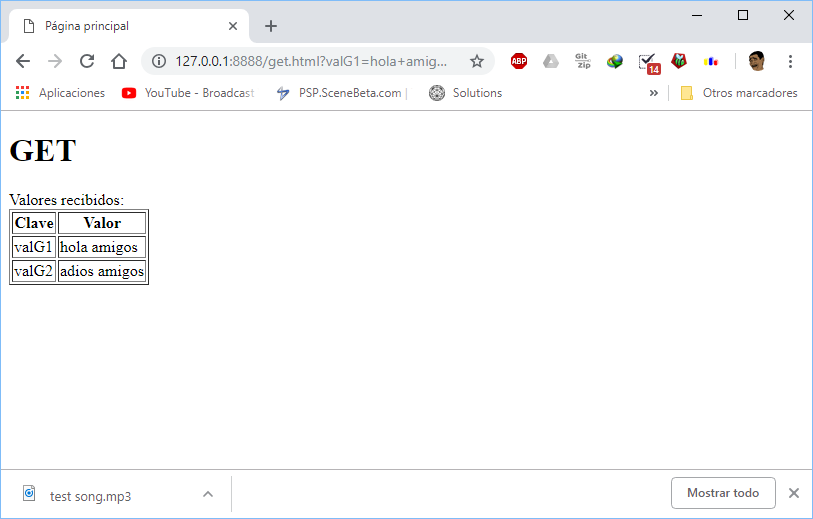
\includegraphics[scale=0.85]{prueba6.png}
		\end{figure}
		
		\clearpage
		Prueba del método \texttt{POST}:
		\begin{figure}[H]
			\centering
			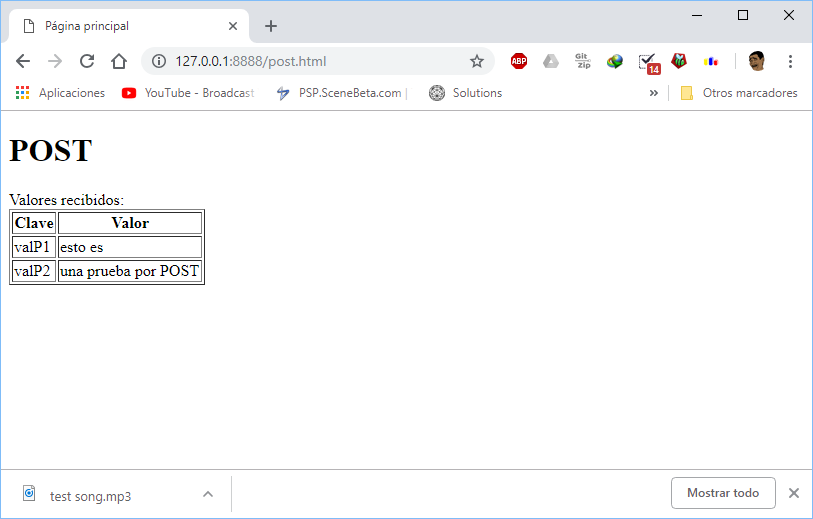
\includegraphics[scale=0.85]{prueba7.png}
		\end{figure}
		
		\clearpage
		Prueba del método \texttt{PUT}
		\begin{figure}[H]
			\centering
			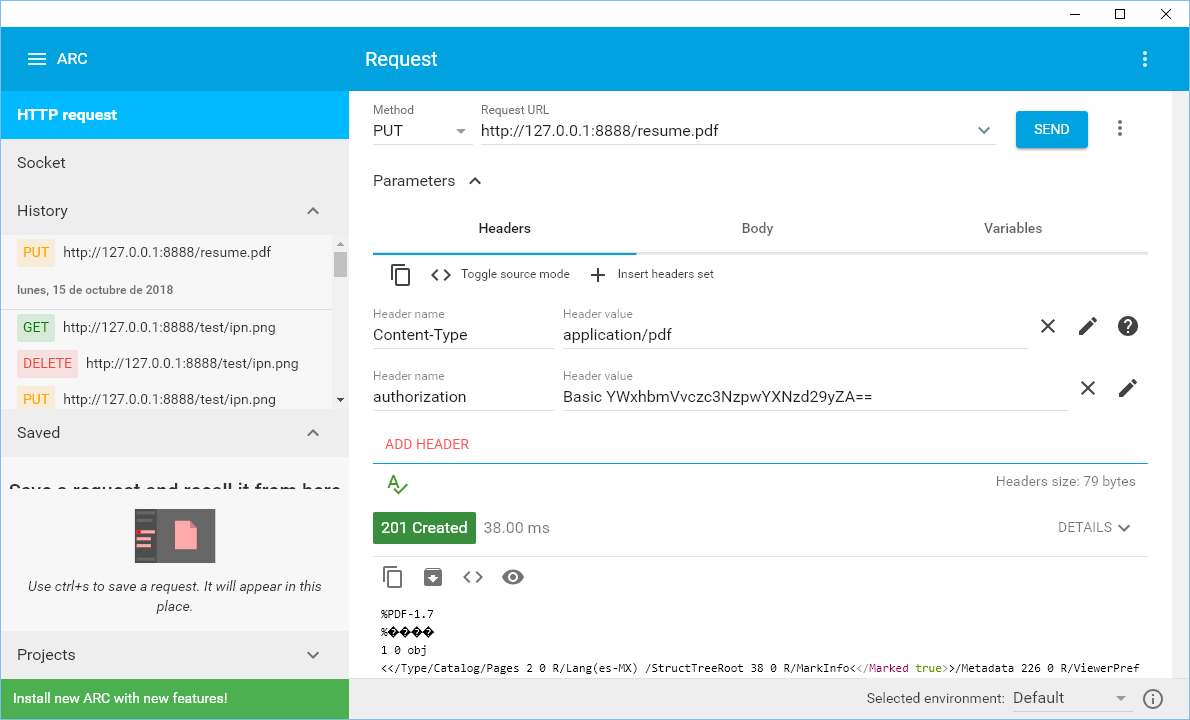
\includegraphics[scale=0.6]{prueba81.png}
		\end{figure}
	
		\begin{figure}[H]
			\centering
			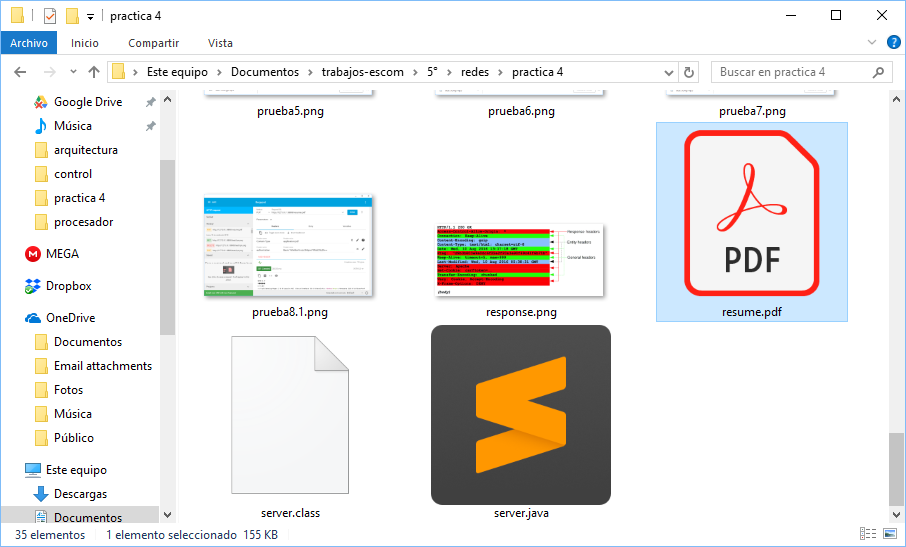
\includegraphics[scale=0.7]{prueba82.png}
		\end{figure}
	
		\clearpage
		Prueba del método \texttt{DELETE}
		\begin{figure}[H]
			\centering
			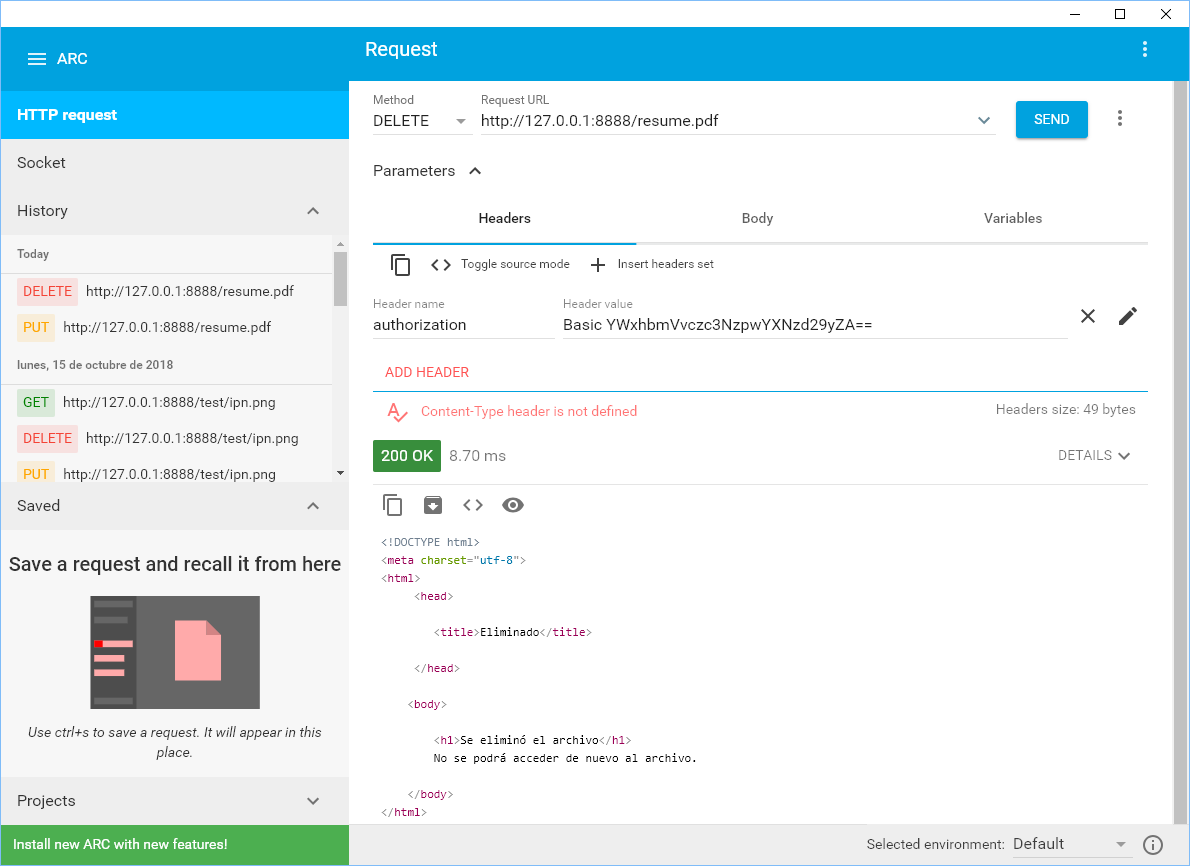
\includegraphics[scale=0.6]{prueba9.png}
		\end{figure}
	
	\clearpage
	\section{Conclusiones}
		En esta práctica implementamos una versión muy sencilla del protocolo HTTP 1.1. Tuvimos que tener un buen manejo de los \texttt{streams} en java y de escribir correctamente los headers y el cuerpo a la salida, tal y como lo dice el protocolo HTTP; y por cada método que íbamos recibiendo, ejecutar las acciones correspondientes, validando todos los posibles códigos de estado de acuerdo a lo que el cliente diga. Usamos expresiones regulares para extraer de forma mucho más sencilla los datos que recibimos de los clientes.
		
		A pesar de ser una versión muy reducida, cumple muy bien con el objetivo de demostrar la implementación del protocolo HTTP desde cero y comprobar que funciona en cualquier navegador, e incluso soporta sustituciones muy básicas de los campos almacenados en el formulario, a través de \texttt{GET} y \texttt{POST}; así como el soporte de un muy básico inicio de sesión mediante el navegador.
		
		Por último, haberlo implementado sobre un pool de conexiones nos da mayor eficiencia, pues no se crea un hilo por cada cliente que va llegando, sino que si se supera el máximo número de clientes simultáneos, tendrán que esperar hasta que uno se desocupe. Pero como HTTP es \emph{stateless}, esto pasa muy rápido y, a menos que un cliente esté descargando algo muy pesado, la asignación de los recursos entre clientes se dará de una forma transparente.
	
	
\end{document}